\RequirePackage{amsmath,mathtools}
\documentclass[a4paper,10pt,department=FakEI]{OTHRartcl}

% ==============================================================================
% PAKETE & EINSTELLUNGEN
% ==============================================================================
\usepackage{iftex}
\ifTUTeX
\else
    \usepackage[utf8]{inputenc}
    \usepackage[T1]{fontenc}
    \usepackage{amssymb}
\fi
\usepackage[ngerman]{babel}
\usepackage{geometry}
\usepackage{graphicx}
\usepackage{booktabs}
\usepackage{tabularx}
\usepackage{array}
\usepackage{xcolor}
\usepackage{float}
\usepackage{tcolorbox}
\tcbuselibrary{skins,breakable}
\usepackage{caption}
\usepackage{listings}
\usepackage{hyperref}
\usepackage[
    headsepline=0.4pt,
    footsepline=0.4pt,
    plainfootsepline=true
]{scrlayer-scrpage}

% Seitengeometrie
\geometry{
    a4paper,
    top=18mm,
    bottom=18mm,
    left=18mm,
    right=18mm,
    headheight=14pt,
    headsep=5mm,
    footskip=8mm
}
\setlength{\footheight}{20pt}

% OTH-Farben
\definecolor{primaryBlue}{RGB}{0, 75, 135}
\definecolor{darkgray}{RGB}{50, 50, 50}
\definecolor{lightgray}{RGB}{246, 248, 251}
\definecolor{accentOrange}{RGB}{235, 115, 35}
\definecolor{codeGreen}{RGB}{20, 120, 40}

% Hyperref Setup
\hypersetup{
    colorlinks=true,
    linkcolor=primaryBlue,
    citecolor=primaryBlue,
    urlcolor=primaryBlue,
    pdftitle={Versuch V3: Reglerentwurf Drosselklappe - Regelungstechnik Anwendungen},
    pdfauthor={Johannes Wutz, Oliver Grundmann, Eduardo Llama}
}

% Bildunterschriften
\captionsetup{
    font={small},
    labelfont={bf,color=primaryBlue},
    labelsep=colon,
    skip=3pt
}

% Tabellenabstände
\renewcommand{\arraystretch}{1.12}

% Boxen-Design
\tcbset{
    enhanced,
    colback=lightgray,
    colframe=primaryBlue!35,
    boxrule=0.6pt,
    arc=1.5mm,
    left=3mm, right=3mm, top=2mm, bottom=2mm
}

% MATLAB Listings
\lstdefinestyle{matlabstyle}{
    language=Matlab,
    basicstyle=\ttfamily\scriptsize,
    backgroundcolor=\color{lightgray},
    frame=single,
    rulecolor=\color{primaryBlue!35},
    keywordstyle=\color{primaryBlue}\bfseries,
    commentstyle=\color{codeGreen},
    numbers=none,
    breaklines=true,
    aboveskip=3pt,
    belowskip=3pt
}

% Kopf- und Fußzeilen
\clearpairofpagestyles
\ihead{\textsf{\small Regelungstechnik Anwendungen $\cdot$ Versuch V3: Reglerentwurf Drosselklappe}}
\ohead{\textsf{\small Gruppe 2}}
\cfoot[\raisebox{-2.5mm}{\textsf{\thepage\ von \pageref*{doc:lastpage}}}]{\raisebox{-2.5mm}{\textsf{\thepage\ von \pageref*{doc:lastpage}}}}
\pagestyle{scrheadings}

% Absatzformatierung
\setlength{\parindent}{0pt}
\setlength{\parskip}{2.5pt}

% Inhaltsverzeichnis Konfiguration
\setcounter{tocdepth}{2}
\setcounter{secnumdepth}{2}
\addto\captionsngerman{\renewcommand*{\contentsname}{Inhalt}}
\deftocheading{toc}{\noindent{\Large\bfseries #1}\par\vspace{2.5mm}}

\DeclareTOCStyleEntry[
    linefill=\TOCLineLeaderFill,
    beforeskip=2.5pt plus 1pt,
    entrynumberformat=\bfseries,
    entryformat=\bfseries,
    pagenumberformat=\bfseries
]{tocline}{section}

\DeclareTOCStyleEntry[
    linefill=\TOCLineLeaderFill,
    beforeskip=0.5pt,
    indent=1.5em,
    numwidth=2.2em
]{tocline}{subsection}

% ==============================================================================
% DOKUMENTENBEGINN
% ==============================================================================
\begin{document}

% ##############################################################################
% SEITE 1: DECKBLATT
% ##############################################################################
\thispagestyle{plain}

\noindent
\begin{minipage}[c]{0.55\textwidth}
    \TheLogo
\end{minipage}%
\begin{minipage}[c]{0.45\textwidth}
    \raggedleft
    {\fontsize{13}{16}\selectfont\bfseries Regelungstechnik Anwendungen}\\[1.5mm]
    {\normalsize Prof. Dr. Brüdigam}
\end{minipage}

\vspace{7mm}

\begin{center}
    {\fontsize{18}{22}\selectfont\bfseries Versuch V3: Reglerentwurf Drosselklappe}
\end{center}

\vspace{4mm}

\begin{tcolorbox}[
    sharp corners,
    colback=white,
    colframe=black,
    boxrule=0.7pt,
    left=8mm, right=8mm, top=5.5mm, bottom=5.5mm
]
\fontsize{10.5}{16}\selectfont
\noindent
Studiengang:\,\underline{\makebox[5.6cm][l]{\strut\hspace{1.5mm}\textbf{Elektro- und Informationstechnik}}}
\hspace{9mm}
Versuchsdatum:\,\underline{\makebox[3.0cm][l]{\strut\hspace{1.5mm}\textbf{21.11.2026}}}

\vspace{4.5mm}
\noindent
Gruppen-Nr.:\,\underline{\makebox[5.6cm][l]{\strut\hspace{1.5mm}\textbf{2}}}

\vspace{4.5mm}
\noindent
Teilnehmer:\,\underline{\makebox[5.6cm][l]{\strut\hspace{1.5mm}\textbf{Johannes Wutz}}}

\vspace{2.8mm}
\noindent
\hphantom{Teilnehmer:\,}\underline{\makebox[5.6cm][l]{\strut\hspace{1.5mm}\textbf{Oliver Grundmann}}}

\vspace{2.8mm}
\noindent
\hphantom{Teilnehmer:\,}\underline{\makebox[5.6cm][l]{\strut\hspace{1.5mm}\textbf{Eduardo Llama}}}
\end{tcolorbox}

\vspace{5mm}

\begingroup
\hypersetup{linkcolor=black}
\tableofcontents
\endgroup

\clearpage

% ##############################################################################
% SEITE 2: GRUNDLAGEN, MITSCHRIFTEN AUS V2 & VORBEREITUNG (KAP. 1)
% ##############################################################################
\section{Grundlagen und Vorbereitung (inkl. Mitschriften aus V2)}

\subsection{Anforderungen an die Drosselklappenlageregelung (Kap.~1.3)}
Für die elektrisch betätigte Drosselklappe (E-Gas) eines Ottomotors gelten folgende Anforderungen:
\begin{itemize}\setlength{\itemsep}{2pt}
    \item \textbf{Genauigkeit:} Sehr hohe stationäre Genauigkeit ($e_{\infty} \to 0^\circ$, Toleranz $< 0{,}2^\circ$). Bereits kleinste Winkelabweichungen verändern im Leerlauf- und Teillastbereich den Luftmassenstrom merklich und führen zu Drehzahlschwankungen oder erhöhten Emissionen.
    \item \textbf{Überschwingen:} Minimales bzw.\ kein Überschwingen ($D \ge 1$). Ein Überschwingen nahe der Endlagen ($0^\circ$ bzw.\ $90^\circ$) führt zu hartem mechanischem Anschlagen (Gefahr von Getriebeschäden), erzeugt Drehmomentstöße im Fahrzeug und provoziert wegen des Vorzeichenwechsels der Geschwindigkeit ein Hängenbleiben in der Haftreibung.
    \item \textbf{Geschwindigkeit:} Sehr hohe Stellgeschwindigkeit (Ausregelzeit $t_{\text{ein}} \approx 50\dots 150\,\text{ms}$), damit der Motor verzögerungsfrei auf Gaspedalbefehle sowie schnelle Momenteneingriffe (ESP/ASR, Leerlaufregelung) reagiert.
\end{itemize}

\subsection{Übernahme der Messwerte und Mitschriften aus Versuch V2}
In Versuch V2 wurden an der realen Drosselklappe (Hebelarm $r = 29{,}35\,\text{mm}$, Getriebe $i = 20 \Rightarrow K_{\text{Gr}} = 0{,}05$, Notlaufposition $\phi_0 = 7{,}5^\circ$ bzw.\ $5^\circ$ im V3-Muster) die nichtlinearen Kennlinien bestimmt:
\begin{table}[H]
\centering
\scriptsize
\caption{Zusammenfassung der Messwerte aus Versuch V2 (\texttt{v2.docx}, \texttt{Mappe1.xlsx}, \texttt{EI7\_V2.slx}) und der V3-Musterparameter.}
\label{tab:v2_parameter}
\begin{tabular*}{\textwidth}{@{\extracolsep{\fill}}llll@{}}
\toprule
\textbf{Teilmodell / Größe} & \textbf{Messwerte aus V2 (bezogen auf Klappe)} & \textbf{Eigenes V2-Modell (\texttt{EI7\_V2.slx})} & \textbf{V3-Laborvorlage (\texttt{TF\_DK\_Stud.m})} \\
\midrule
\textbf{Ankerkreis ($R_A, T_{\text{el}}$)} & $R_A \approx 10\,\Omega$ (Schätzwert Vorber.) & $1/R_A = 0{,}1\,\text{A/V}$, $T_{\text{el}} = 0{,}5\,\text{ms}$ & $1/R_A = 0{,}4\,\text{A/V}$ ($2{,}5\,\Omega$), $T_{\text{el}} = 0{,}6\,\text{ms}$ \\
\textbf{Motorkonstante $k_{\text{Mot}}$} & $0{,}44\,\text{A}$ bei $3\,\text{N} \Rightarrow k_{m,\text{DK}} = 0{,}20\dots 0{,}30\,\text{Nm/A}$ & $k_1 = k_2 = 0{,}045\,\text{Nm/A}$ (Motor) & $F_2 = F_4 = 0{,}03\,\text{Nm/A}$ (Motor) \\
\textbf{Trägheit \& Getriebe} & Untersetzung $i = 20$ ($K_{\text{Gr}} = 0{,}05$) & $J = 2{,}5\cdot 10^{-5}\,\text{kg\,m}^2$, $K_{\text{Gr}} = 0{,}05$ & $J = 8\cdot 10^{-6}\,\text{kg\,m}^2$, $K_{\text{Gr}} = 0{,}05$ \\
\textbf{Notlauffeder $M_F(\phi)$} & $F_F(7{,}5^\circ)=4{,}5\,\text{N}$ ($132\,\text{mNm}$); $c_F = 1{,}24\,\text{mNm/}^\circ$ & $\phi_0 = 7^\circ$, $k_4 = 0{,}0018\,\text{Nm/}^\circ$ & $\phi_0 = 5^\circ$, Sprung $\pm 0{,}025\,\text{Nm}$ am Motor \\
\textbf{Reibmoment $M_R$} & $F_R = F_{\text{ges}}-F_F \approx 9{,}67\,\text{N} \Rightarrow M_{R,\text{DK}} = 283{,}6\,\text{mNm}$ & $k_3 = 0{,}002\,\text{Nm}\cdot\operatorname{sign}(\omega)$ & Coulomb-Lookup: $\pm 0{,}01\,\text{Nm}$ am Motor \\
\bottomrule
\end{tabular*}
\end{table}

\subsection{MATLAB m-File \texttt{TF\_DK\_Stud.m}: Lineare Streckenübertragungsfunktion}
Unter Vernachlässigung der Nichtlinearitäten (Feder und Reibung) ergibt sich die lineare Strecke $F_{12345}(s) = \frac{\Phi_{\text{DK,deg}}(s)}{U_{\text{Mot}}(s)}$:
\begin{lstlisting}[style=matlabstyle]
z_1 = [0.4];      n_1 = [0.0006 1];    F1 = tf(z_1, n_1)          % Anker (R, L): Spannung -> Strom
F2  = 0.03                                                        % Strom -> Motormoment k_Mot
z_3 = [1];        n_3 = [8e-6 0];      F3 = tf(z_3, n_3)          % Moment -> Winkelgeschwindigkeit (1 / (J*s))
F123  = F1 * F2 * F3                                              % Reihenschaltung Vorwaertszweig
F4    = 0.03                                                      % Gegen-EMK Faktor k_EMK
F1234 = feedback(F123, F4)                                        % Geschlossene Motorschleife (EMK-Gegenkopplung)
z_5 = [0.05 * 180 / pi];  n_5 = [1 0]; F5 = tf(z_5, n_5)          % omega -> Motorwinkel -> Klappenwinkel in Grad
F12345 = F1234 * F5                                               % Gesamtstrecke ohne Regler
\end{lstlisting}
Mit den Zahlenwerten der Vorlage folgt die $\text{IT}_2$-Streckenübertragungsfunktion:
\begin{equation}
    F_{12345}(s) = \frac{0{,}03438}{4{,}8\cdot 10^{-9}\,s^3 + 8\cdot 10^{-6}\,s^2 + 0{,}00036\,s} \quad\Longrightarrow\quad s_{P1} = 0,\;\; s_{P2} = -46{,}29\,\text{s}^{-1},\;\; s_{P3} = -1620{,}4\,\text{s}^{-1}
\end{equation}

\clearpage

% ##############################################################################
% SEITE 3: REGELKREIS MIT P-REGLER (KAP. 2.3 & 2.3.1)
% ##############################################################################
\section{Regelkreis mit P-Regler (Kap.~2.3 \& 2.3.1)}

\subsection{Wurzelortskurve und optimale Verstärkung für schnellstes Einschwingen}
Mit einem P-Regler ($F_R(s) = K_P$) wandern die beiden dominanten reellen Pole $s_{P1} = 0$ und $s_{P2} = -46{,}29\,\text{s}^{-1}$ aufeinander zu und treffen sich im Verzweigungspunkt $s_{1,2} = \textbf{-22,98\,s}^{-1}$. Dort liegt der aperiodische Grenzfall ($D = 1$, schnellstes Einschwingen ohne Überschwingen) bei:
\begin{equation}
    K_{P,\text{opt}} = \mathbf{0{,}1195}\,\text{V}/^\circ
\end{equation}

\begin{figure}[H]
\centering

\includegraphics[width=\textwidth,height=5.9cm,keepaspectratio]{plot_v3_wok_p_regler.png}
\caption{Wurzelortskurve des offenen Regelkreises mit P-Regler (\texttt{rlocus(Fo\_P)}): Gesamtansicht (links) und dominanter Bereich (rechts).}
\label{fig:wok_p}
\end{figure}

\subsection{Simulation des nichtlinearen Systems (Sprung \texorpdfstring{$10^\circ \to 60^\circ$}{10 Grad auf 60 Grad}) und Fehleranalyse}
\begin{figure}[H]
\centering

\includegraphics[width=\textwidth,height=5.9cm,keepaspectratio]{plot_v3_sim_p_regler.png}
\caption{Verhalten des P-geregelten, nichtlinearen Systems (\texttt{DK\_V3.slx}) bei einem Sollwertsprung von $10^\circ$ auf $60^\circ$.}
\label{fig:sim_p}
\end{figure}

\begin{itemize}\setlength{\itemsep}{2pt}
    \item \textbf{Erkannte Probleme:} Bei $K_{P,\text{opt}} = 0{,}1195\,\text{V/}^\circ$ bleibt die Klappe bereits bei $\phi_{\infty} = \textbf{36,96}^\circ$ stehen (bleibende Regelabweichung $e_{\infty} = \textbf{23,04}^\circ$). Höhere Verstärkungen reduzieren zwar $e_{\infty}$ ($K_P = 0{,}5 \Rightarrow \phi_{\infty} = 55{,}6^\circ$; $K_P = 2{,}0 \Rightarrow \phi_{\infty} = 58{,}85^\circ$), führen ab $K_P > 0{,}5$ aber zu komplexen Polen ($D < 1$) und deutlichem Überschwingen ($\phi_{\max} = 64{,}3^\circ$ bei $K_P = 2{,}0$).
    \item \textbf{Ursachen:} Die stark vorgespannte Notlauffeder ($M_F \approx 0{,}0276\,\text{Nm}$ bei $60^\circ$) und die Coulomb-Reibung ($M_R = \pm 0{,}01\,\text{Nm}$) greifen \emph{vor} dem Streckenintegrator an. Allein zum Halten gegen die Feder benötigt der Motor bei $60^\circ$ einen Dauerstrom $I_{\text{halt}} = M_F / k_{\text{Mot}} = 0{,}92\,\text{A}$ bzw.\ eine Dauerspannung $U_{\text{halt}} = R_A \cdot I_{\text{halt}} \approx \textbf{2,30\,V}$. Da beim P-Regler $U_{\text{Mot}} = K_P \cdot e$ gilt, bleibt die Klappe stehen, sobald $K_P \cdot e \le (M_F + M_R)\cdot R_A / k_{\text{Mot}}$ erreicht ist.
    \item \textbf{Verbesserung und geeignete Regler:} Ein reiner P-Regler kann die Anforderungen nicht gleichzeitig erfüllen (bester P-Kompromiss: $K_P \approx 0{,}4\dots 0{,}5\,\text{V/}^\circ$). Um die stationäre Federkraft bei $e_{\infty} = 0$ zu kompensieren, ist zwingend ein \textbf{I-Anteil} nötig; wegen der beiden Integratoren im offenen Kreis ($s_{P1,2} = 0$) muss dieser mit einem \textbf{D-Anteil} zur Stabilisierung und Beschleunigung kombiniert werden ($\Rightarrow$ \textbf{$\text{PIDT}_1$-Regler}).
\end{itemize}

\clearpage

% ##############################################################################
% SEITE 4: PIDT1-REGLER & VERSUCHSAUSWERTUNG (KAP. 2.3.2 & KAP. 3)
% ##############################################################################
\section{\texorpdfstring{$\text{PIDT}_1$}{PIDT1}-Regler und Versuchsauswertung (Kap.~2.3.2 \& Kap.~3)}

\subsection{Auslegung des \texorpdfstring{$\text{PIDT}_1$}{PIDT1}-Reglers über Nullstellenvorgabe}
Für den Simulink-$\text{PIDT}_1$-Regler gilt mit gewählter Filterzeitkonstante $T = 1/N = 0{,}001\,\text{s}$ und den gewünschten Nullstellen $s_{N1} = -10\,\text{s}^{-1}$, $s_{N2} = -30\,\text{s}^{-1}$ (mit $(s+10)(s+30) = s^2 + 40s + 300$):
\begin{equation}
    F_R(s) = K\left(1 + \frac{1}{T_N s} + \frac{T_V s}{T s + 1}\right) = K\,\frac{(T T_N + T_N T_V)s^2 + (T + T_N)s + 1}{T T_N s^2 + T_N s} \;\stackrel{!}{=}\; K\,\frac{Q\,(s+10)(s+30)}{T T_N s^2 + T_N s}
\end{equation}
Durch Koeffizientenvergleich folgt $Q = \frac{1}{300}$, $T + T_N = \frac{40}{300} \Rightarrow T_N = \textbf{0,13233\,s}$ und $T T_N + T_N T_V = \frac{1}{300} \Rightarrow T_V = \textbf{0,02419\,s}$. In der WOK (Abbildung~\ref{fig:wok_pidt1}) münden die aus $s_{P1,2} = 0$ startenden Äste bei $s = -16{,}4\,\text{s}^{-1}$ wieder auf die reelle Achse ein ($D = 1$ bei $K_{\text{WOK}} = \textbf{0,0695}$; Simulink-Parallelform: $P = 0{,}0695$, $I = K/T_N = 0{,}5252\,\text{s}^{-1}$, $D = K T_V = 0{,}001681\,\text{s}$, $N = 1/T = 1000\,\text{s}^{-1}$).

\begin{figure}[H]
\centering
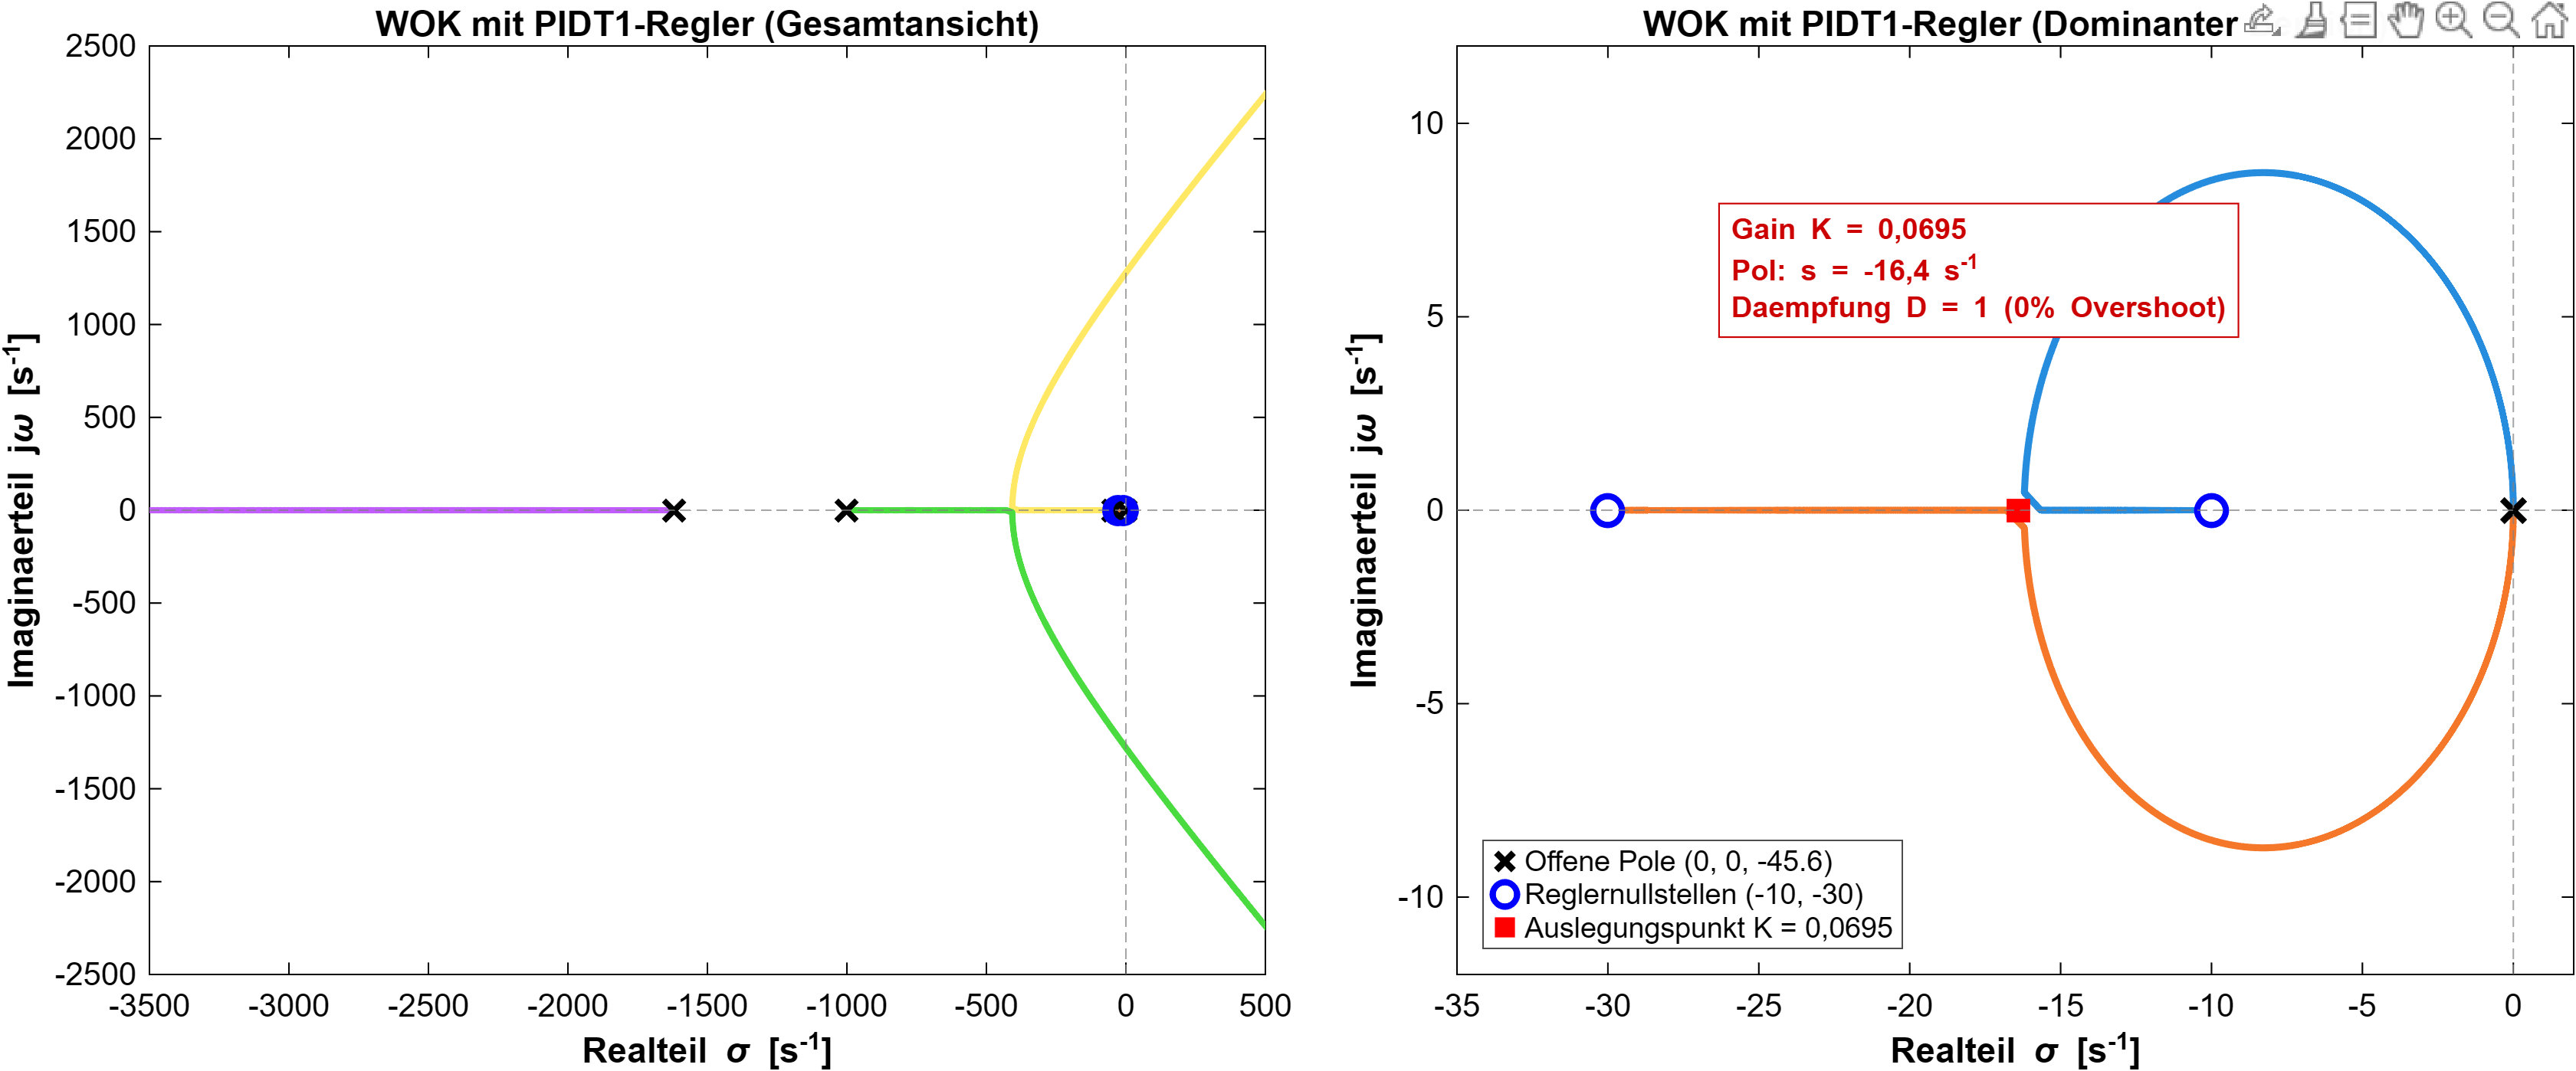
\includegraphics[width=\textwidth,height=4.0cm,keepaspectratio]{plot_v3_wok_pidt1_regler.png}
\caption{Wurzelortskurve des offenen Regelkreises mit $\text{PIDT}_1$-Regler: Gesamtansicht (links) und dominanter Bereich um $s = -16{,}4\,\text{s}^{-1}$ (rechts).}
\label{fig:wok_pidt1}
\end{figure}

\subsection{Simulation, Reglervergleich und Verbesserungsvorschläge (Kap.~3)}
\begin{figure}[H]
\centering
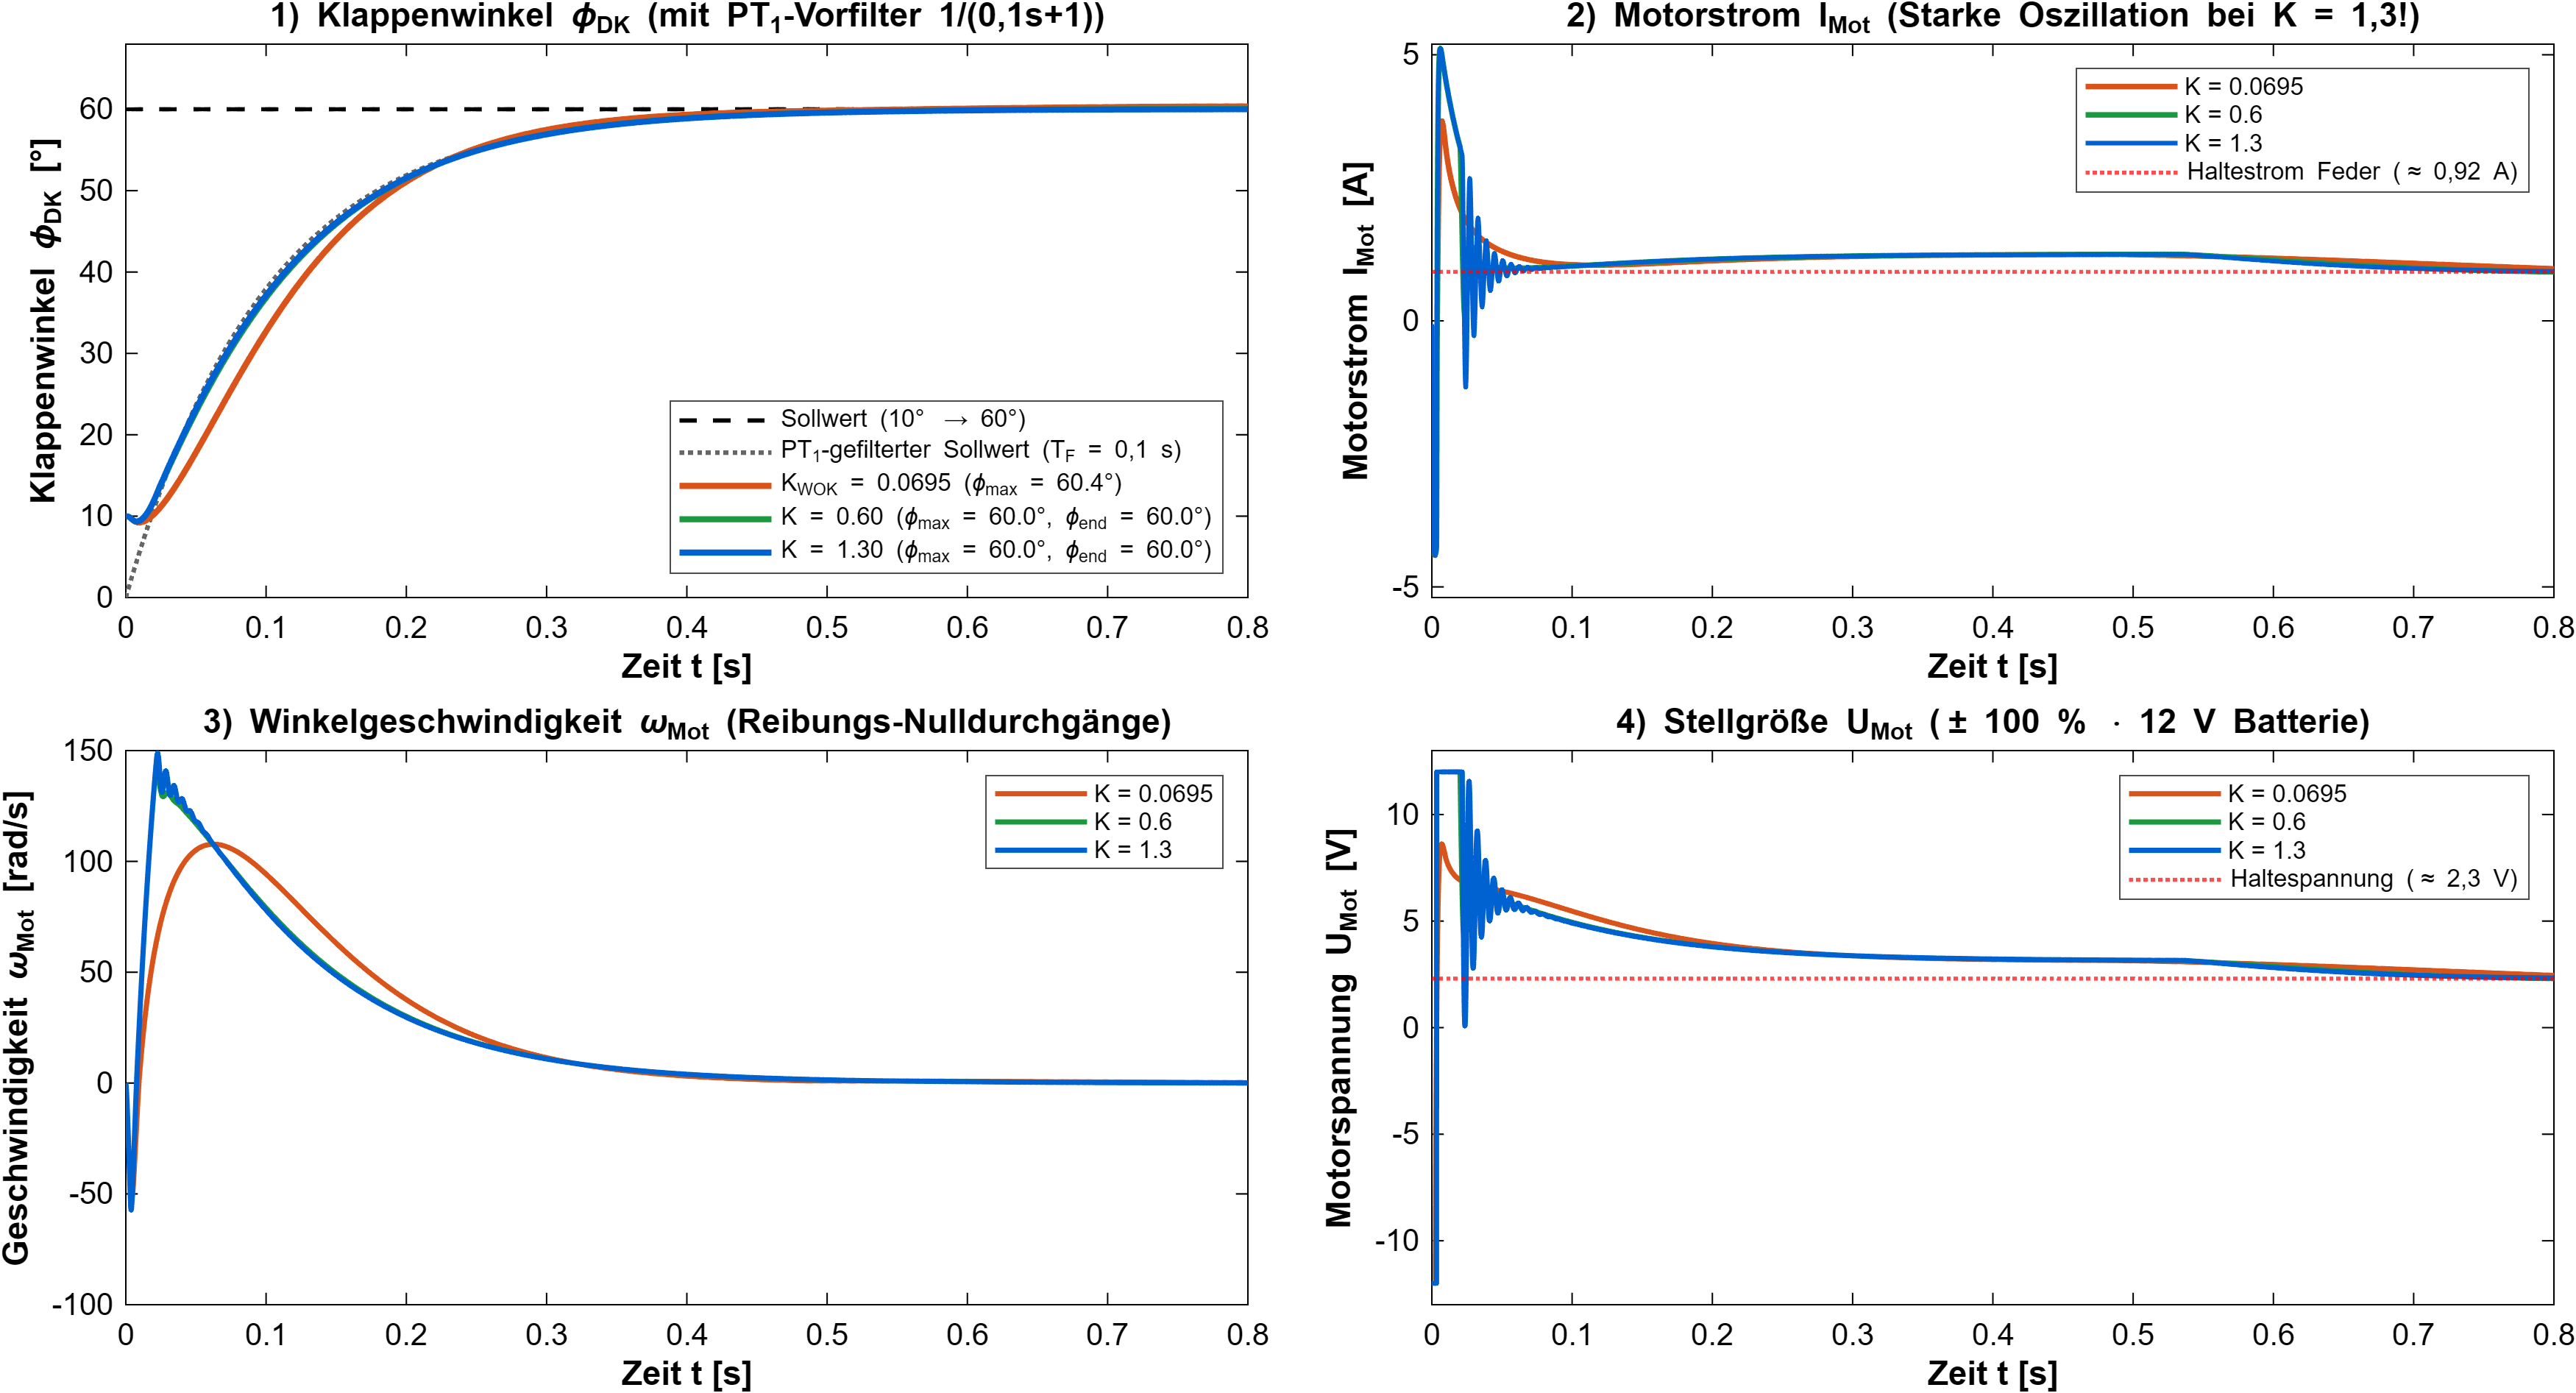
\includegraphics[width=\textwidth,height=4.0cm,keepaspectratio]{plot_v3_sim_pidt1_regler.png}
\caption{Simulation des $\text{PIDT}_1$-geregelten Systems beim Sprung $10^\circ \to 60^\circ$ für verschiedene Verstärkungen $K$ sowie mit $\text{PT}_1$-Führungsgrößenfilter ($1/(0{,}1s+1)$) und Anti-Windup.}
\label{fig:sim_pidt1}
\end{figure}

\begin{itemize}\setlength{\itemsep}{1pt}
    \item \textbf{Warum sind die Ergebnisse mit $K = 0{,}0695$ nicht optimal? Erklären der Auffälligkeiten:}
    Obwohl die lineare WOK für $K = 0{,}0695$ exakt $D = 1$ ($0\,\%$ Overshoot) vorhersagt, schwingt die nichtlineare Klappe bis auf $\phi_{\max} = \textbf{71,5}^\circ$ über und kriecht danach extrem langsam Richtung $60^\circ$ zurück (bei $t = 1{,}5\,\text{s}$ erst auf $56{,}8^\circ$). \textbf{Ursachen:} 1.~Die langsame Reglernullstelle $s_{N1} = -10\,\text{s}^{-1}$ liegt in der Führungsübertragungsfunktion näher am Ursprung als das dominante Polpaar ($s = -16{,}4\,\text{s}^{-1}$) und erzeugt zusammen mit dem D-Stoß einen starken Überschwinger sowie die sofortige \textbf{Stellgrößensättigung ($+12\,\text{V}$)}, in der der Integrator überlädt (\textbf{Integrator-Windup}). 2.~Nach dem Umkehrpunkt bleibt die Klappe im \textbf{Haft-/Coulomb-Reibungsband ($\pm 0{,}01\,\text{Nm}$)} hängen und kriecht nur im Tempo des kleinen I-Anteils ($I = 0{,}525\,\text{s}^{-1}$) zum Sollwert.
    \item \textbf{Konkrete Verbesserungsvorschläge:}
    1.~\textbf{$\text{PT}_1$-Führungsgrößenfilter (Vorfilter) zur Kompensation der Nullstelle $s_{N1} = -10\,\text{s}^{-1}$:} Durch Vorschalten eines $\text{PT}_1$-Glieds $F_F(s) = \frac{1}{T_F s + 1} = \frac{1}{0{,}1\,s + 1}$ ($T_F = \frac{1}{|s_{N1}|} = 0{,}1\,\text{s}$) direkt nach dem Sollwertsprung wird die überschwingtreibende Reglernullstelle $(0{,}1\,s + 1)$ in der Führungsübertragungsfunktion exakt kompensiert und der aggressive D-Stoß auf $+12\,\text{V}$ beim Sollwertsprung eliminiert.
    2.~\textbf{Anti-Windup (Clamping):} Interne Reglerbegrenzung auf $\pm 12\,\text{V}$ mit Anti-Windup stoppt die Integration in der Sättigung (in Kombination mit dem $\text{PT}_1$-Vorfilter und $K = 0{,}50$ führt dies zu einem nahezu überschwingfreien, schnellen Einregeln auf exakt $60{,}0^\circ$, siehe grüne Kurve).
    3.~\textbf{Vorsteuerung der Notlauffeder:} Aufschalten von $U_{\text{Vor}}(\phi_{\text{soll}}) = \frac{R_A}{k_{\text{Mot}}} M_F(\phi_{\text{soll}}) \approx 2{,}25\,\text{V}$ kompensiert das statische Federmoment direkt.
\end{itemize}

\begin{tcolorbox}[title={\textbf{Gewonnene Erkenntnisse (1 bis 3 Sätze)}}, coltitle=white, colbacktitle=primaryBlue, top=1mm, bottom=1mm]
\footnotesize Ein rein anhand der linearisierten Wurzelortskurve ausgelegter Regler weicht an der realen Drosselklappe aufgrund des Vorspannungssprungs der Notlauffeder, der Haftreibung, der dominanten Reglernullstelle bei $-10\,\text{s}^{-1}$ und der $+12\,\text{V}$-Stellgrößenbegrenzung stark vom linearen Idealverhalten ab (hohe bleibende Abweichung beim P-Regler bzw.\ Überschwingen und Reibungs-Kriechen beim $\text{PIDT}_1$-Regler). Erst der I-Anteil des $\text{PIDT}_1$-Reglers kann das permanente Federrückstellmoment stationär auf $e_{\infty} = 0^\circ$ ausregeln, wobei für ein schnelles und überschwingfreies Verhalten zusätzlich ein \textbf{$\text{PT}_1$-Führungsgrößenfilter} (zur Kompensation der Nullstelle bei $-10\,\text{s}^{-1}$), \textbf{Anti-Windup} sowie eine \textbf{Vorsteuerung der Federkennlinie} eingesetzt werden sollten.
\end{tcolorbox}

\clearpage

% ##############################################################################
% SEITE 5: BEANTWORTUNG DER TESTFRAGEN (KAP. 4)
% ##############################################################################
\section{Beantwortung der Testfragen (Kap.~4)}
\vspace{-2mm}
\subsection{Wurzelortskurve und MATLAB-Befehle für \texorpdfstring{$s_{P1} = s_{P2} = 0;\; s_{P3} = -3;\; s_{N1} = -1$}{sP1=sP2=0, sP3=-3, sN1=-1}}
\begin{minipage}[c]{0.55\textwidth}
    \footnotesize
    \textbf{Konstruktion der WOK:}
    \begin{itemize}\setlength{\itemsep}{1pt}
        \item \textbf{Reelle Achse:} Ungerade Anzahl an Polen + Nullstellen rechts davon liegt nur im Intervall $[-3, -1]$ vor (2 Pole bei $0$ + 1 Nullstelle bei $-1 \Rightarrow 3$). Somit wandert $s_{P3} = -3$ auf der reellen Achse direkt in die Nullstelle $s_{N1} = -1$.
        \item \textbf{Asymptoten ($n - m = 3 - 1 = 2$):} Winkel $\phi_A = \frac{\pm 180^\circ}{2} = \pm 90^\circ$; Schnittpunkt auf der reellen Achse: $\sigma_A = \frac{(0 + 0 - 3) - (-1)}{3 - 1} = \frac{-2}{2} = -1$. Die beiden Pole aus $s_{P1,2} = 0$ verzweigen sofort ins Komplexe und nähern sich für $K \to \infty$ der Vertikalen $\sigma_A = -1$ nach $\pm j\infty$ an.
    \end{itemize}
    \textbf{Zugehörige MATLAB-Befehle:}
\begin{lstlisting}[style=matlabstyle]
Fo = tf([1 1], [1 3 0 0]);   % Variante 1: (s+1)/(s^3 + 3*s^2)
% Fo = zpk([-1], [0 0 -3], 1); % Variante 2: Pol-/Nullstellenform
rlocus(Fo); grid on;
\end{lstlisting}
\end{minipage}\hfill
\begin{minipage}[c]{0.42\textwidth}
    \centering
    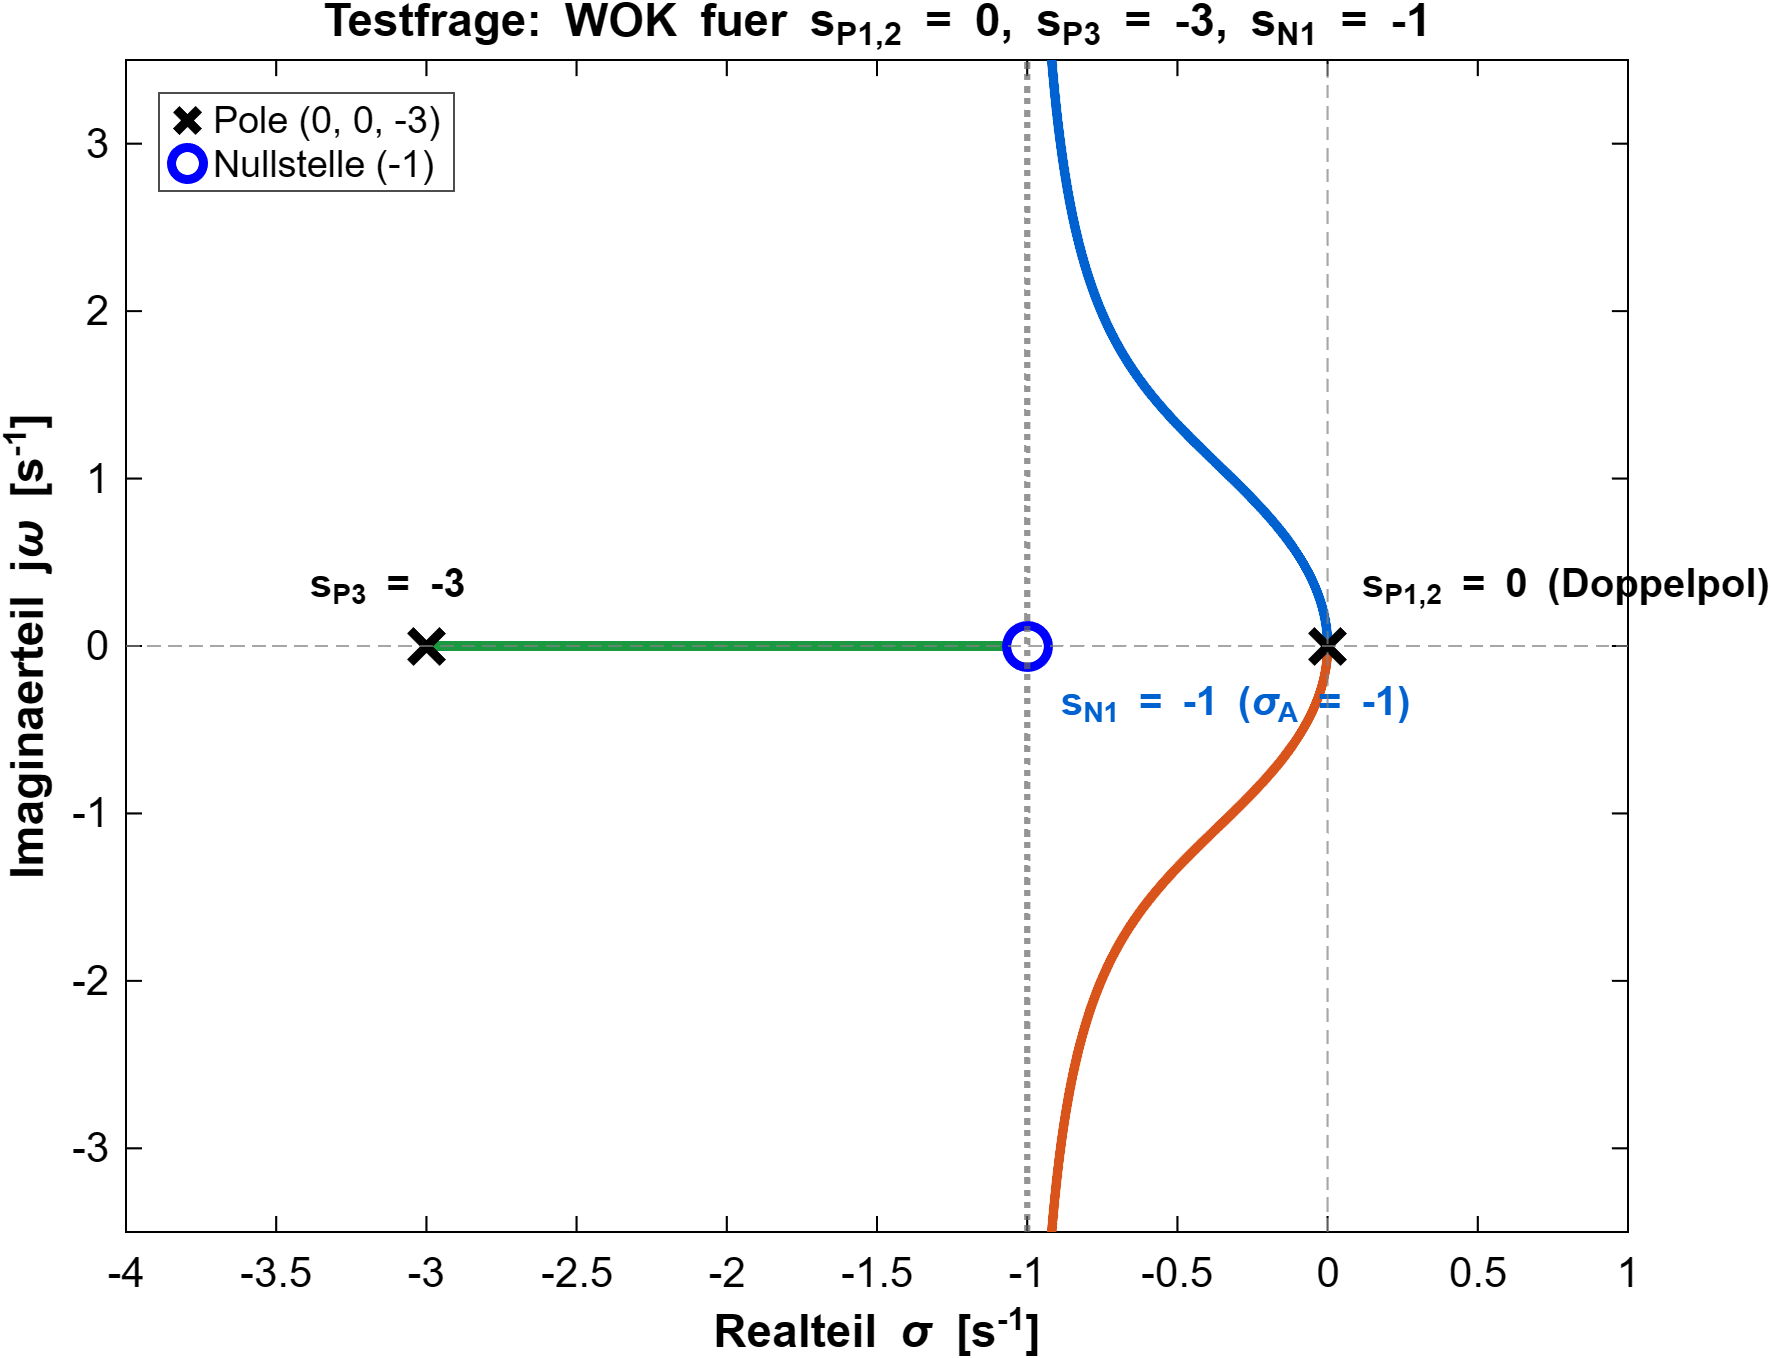
\includegraphics[width=\textwidth,height=3.6cm,keepaspectratio]{plot_v3_testfrage_wok.png}
    \captionof{figure}{WOK für $s_{P1,2}=0$, $s_{P3}=-3$, $s_{N1}=-1$.}
    \label{fig:test_wok}
\end{minipage}

\vspace{-2mm}
\subsection{Bedeutung von Pol- und Nullstellen sowie Pol-/Nullstellenkompensation}
\footnotesize
\begin{itemize}\setlength{\itemsep}{1pt}
    \item \textbf{Bedeutung von Polstellen ($N(s) = 0$):} Bestimmen die \textbf{Stabilität} und die Zeitkonstanten bzw.\ Eigenfrequenzen der freien Eigenbewegungen $e^{s_{Pi} t}$. Es gilt: $\operatorname{Re}\{s_{Pi}\} < 0$ (stabil, klingt umso schneller ab, je weiter links), $\operatorname{Re}\{s_{Pi}\} = 0$ (grenzstabil), $\operatorname{Re}\{s_{Pi}\} > 0$ (instabil); $\operatorname{Im}\{s_{Pi}\} \neq 0$ kennzeichnet schwingungsfähige konjugiert-komplexe Polpaare.
    \item \textbf{Bedeutung von Nullstellen ($Z(s) = 0$):} Bestimmen die Anregungsstärke (Gewichtung) der Eigenmoden im Zeitsignal (differenzierender Phasenvorhalt) und bilden in der Wurzelortskurve die \textbf{Endpunkte (Attraktoren)}, zu denen die geschlossenen Regelkreispole für $K \to \infty$ hinwandern.
    \item \textbf{Pol-/Nullstellenkompensation:} Gezieltes Platzieren einer Reglernullstelle exakt auf einem langsamen, stabilen Streckenpol ($s_{N,\text{Regler}} = s_{P,\text{Strecke}}$), sodass sich beide Linearfaktoren im offenen Kreis $F_o(s) = F_R(s) F_S(s)$ herauskürzen. Dadurch wird die träge Streckenzeitkonstante kompensiert und der Regelkreis beschleunigt (darf niemals bei instabilen Polen angewendet werden!).
\end{itemize}

\vspace{-2mm}
\subsection{Pole, Nullstellen und Sprungantwort von \texorpdfstring{$\text{PT}_1$-, $\text{PD}$- und $\text{PDT}_1$-Glied}{PT1-, PD- und PDT1-Glied}}
\begin{figure}[H]
\centering
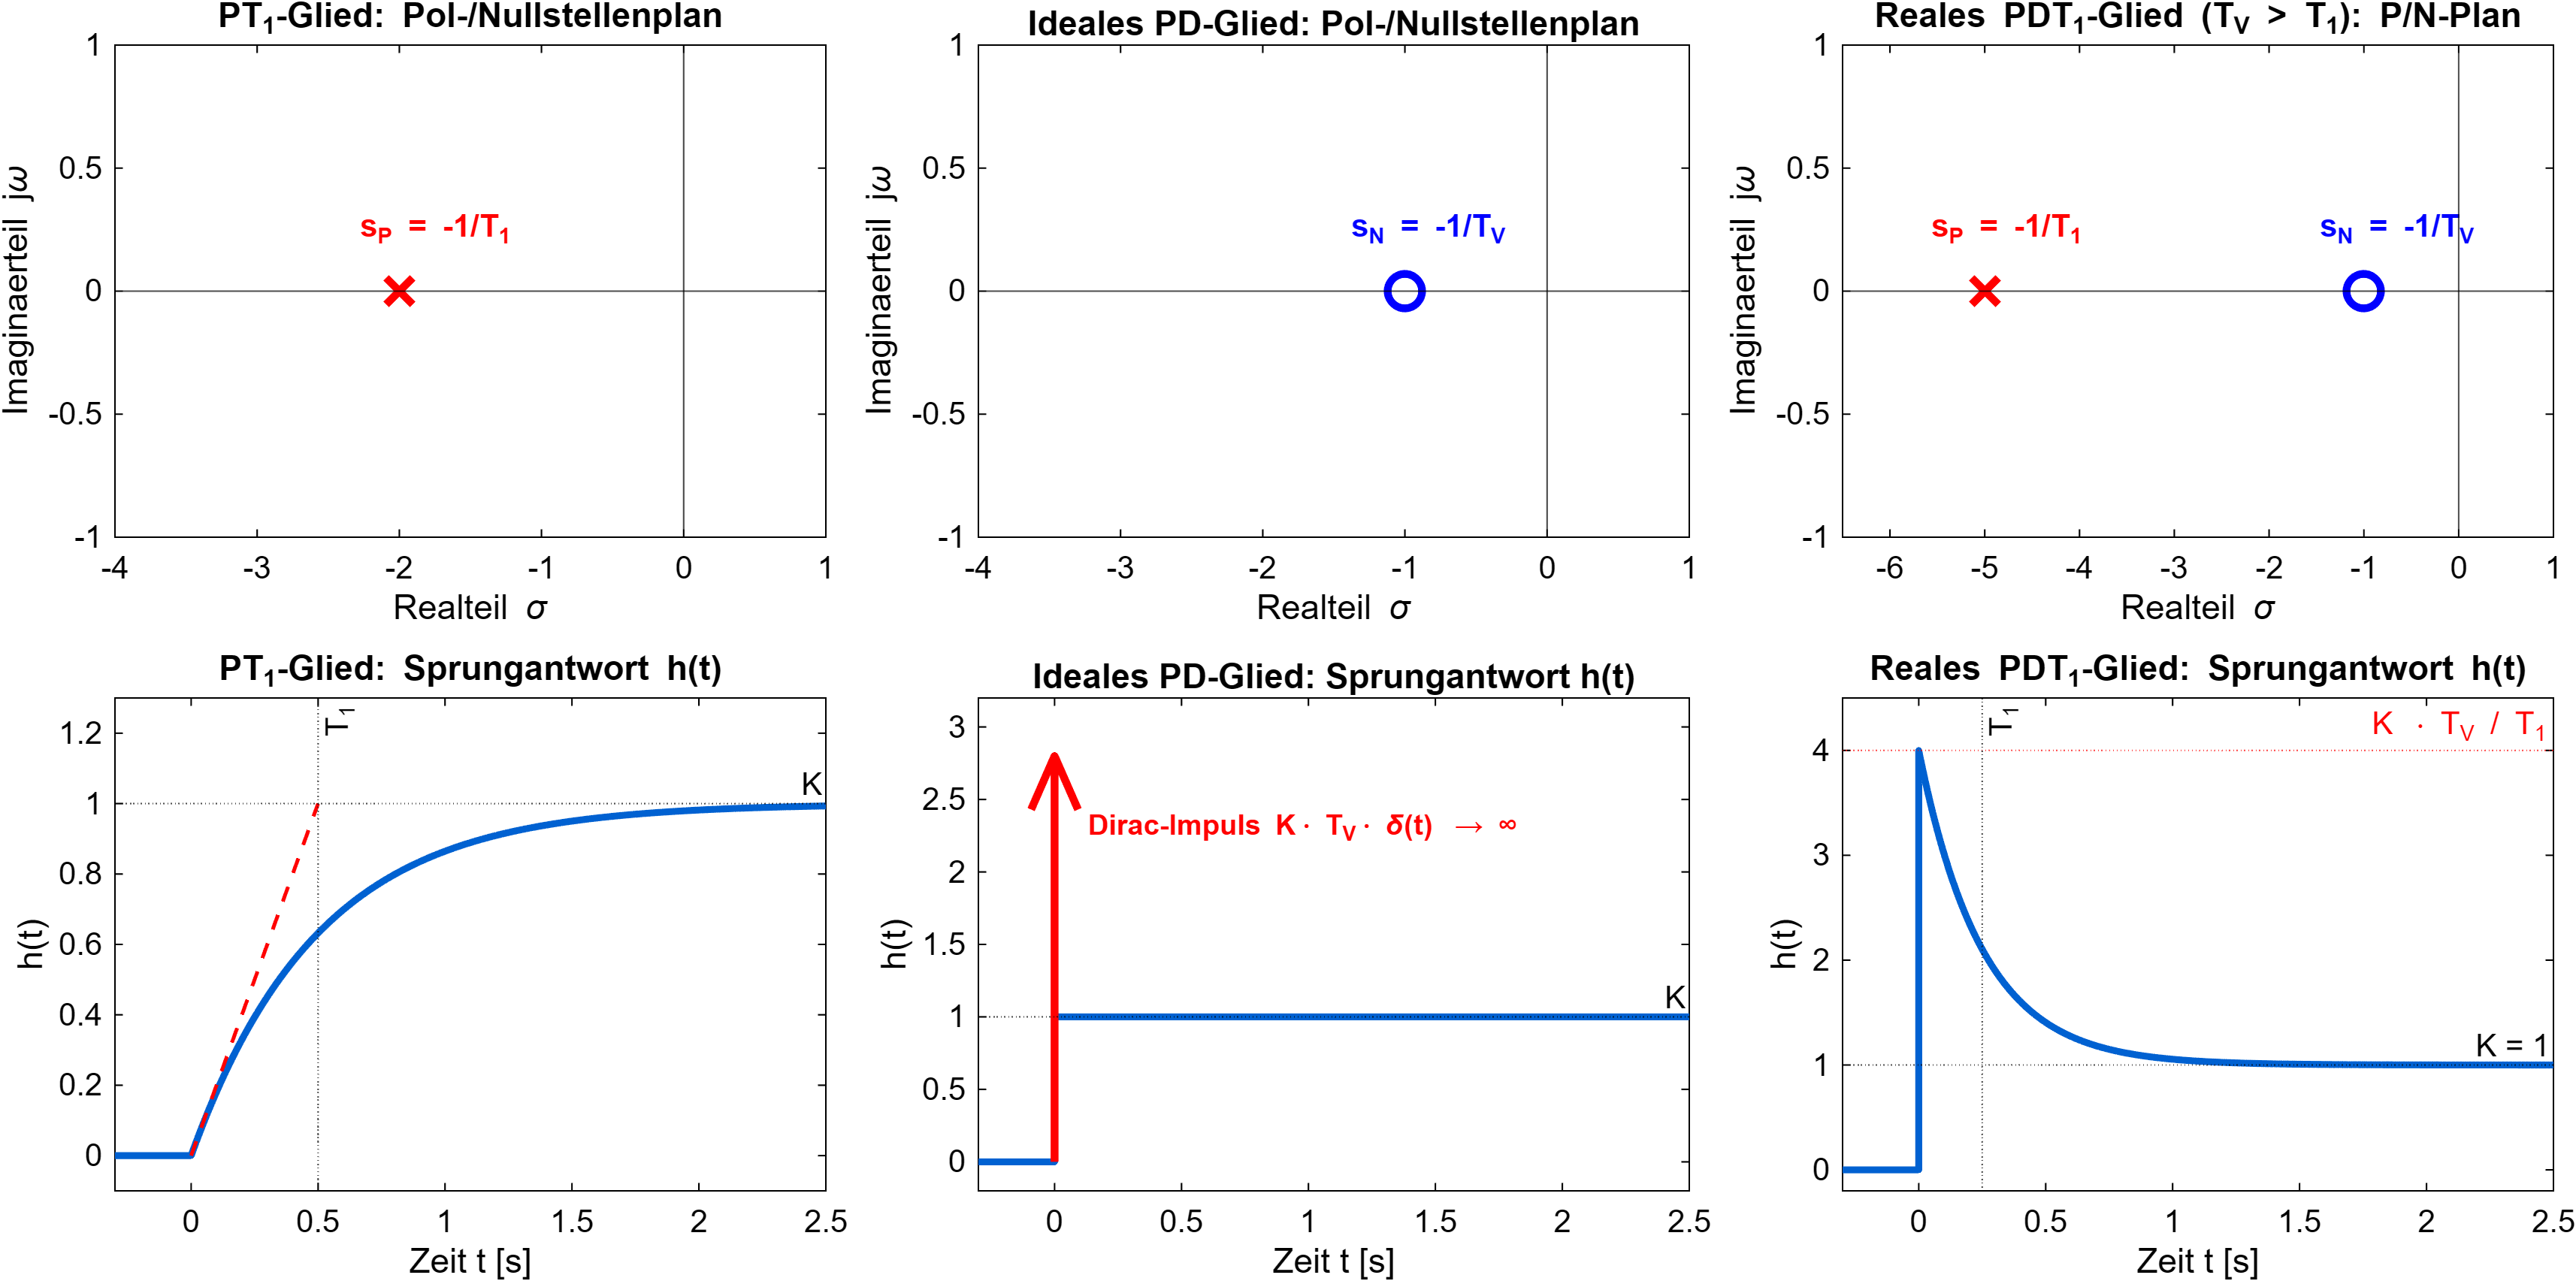
\includegraphics[width=\textwidth,height=3.5cm,keepaspectratio]{plot_v3_testfrage_glieder.png}
\caption{Pol-/Nullstellenpläne (oben) und zugehörige Sprungantworten $h(t)$ (unten) von $\text{PT}_1$-, idealem $\text{PD}$- und realem $\text{PDT}_1$-Glied.}
\label{fig:test_glieder}
\end{figure}

\vspace{-3mm}
\subsection{Bestimmung von \texorpdfstring{$T_N$ und $T_V$}{TN und TV} eines \texorpdfstring{$\text{PIDT}_1$}{PIDT1}-Reglers aus vorgegebenen Nullstellen}
\footnotesize
Man bringt die Übertragungsfunktion des $\text{PIDT}_1$-Reglers auf den Hauptnenner $F_R(s) = K\,\frac{(T T_N + T_N T_V)s^2 + (T + T_N)s + 1}{T T_N s^2 + T_N s}$ und setzt das Zählerpolynom mit dem normierten Wunschpolynom der beiden Nullstellen $Q\,(s - s_{N1})(s - s_{N2}) = Q\,\big(s^2 - (s_{N1}+s_{N2})s + s_{N1} s_{N2}\big)$ gleich. Bei fest gewählter kleiner Filterzeitkonstante $T$ (z.B.\ $1\,\text{ms}$) liefert der Koeffizientenvergleich nacheinander: 1.~$Q = \frac{1}{s_{N1} s_{N2}}$ (aus $s^0$), 2.~$T_N = -Q\,(s_{N1}+s_{N2}) - T$ (aus $s^1$) und 3.~$T_V = \frac{Q - T\cdot T_N}{T_N}$ (aus $s^2$).

\label{doc:lastpage}
\end{document}
